\documentclass{beamer}

\usetheme{Berlin}


\begin{document}
  
  \title[Grammar of Tables]{Grammar of Tables}
  \subtitle{Reproducible Research}
  \author[S. Garbett, T. Stewart]{S. Garbett \and T. Stewart}
  \date[]{May 17th, 2016: Progress Report}
  
  \frame{\titlepage}
  \begin{frame}
    \frametitle{Original Project Goal}
    \begin{itemize}
    \item To provide an index to numeric data in a statistical report.
    \end{itemize}
    The essential goal is to provide indexing into numerical summary tables
    that are provided as part of \texttt{Hmisc}.
  \end{frame}
  \begin{frame}
    \frametitle{Expanded Project Goal}
    \framesubtitle{And it all got bigger}
    The extensibility of \texttt{summaryM} to include a variety of different or alternate methods in table generation is limited. The idea that a newer table summary generator, that is compatible with \texttt{summaryM} and could generate the required indexes is envisioned. Could one define a grammar of tables in a similar manner to \texttt{ggplot}?
 \end{frame}
 \begin{frame}
   \frametitle{Project Requirement}
   \begin{enumerate}
     \item It must render to LaTeX, Text, HTML5, RMarkdown, Index table.
     \item It must allow for user override of any derivation function.
     \item It must allow for user override of any rendering function.
     \item It must be easily extensible. I.e., any user overrides should require a minimum of fuss / syntax for the end user.
     \item Index table must be user specified name based, and not numeric numbers.
     \item Index table must be repeatible, and contain search information.
     \item It should reproduce by default, Hmisc summaryM behaviors.
   \end{enumerate}
  \end{frame}
    \begin{verbatim}

functionDefaults = list(factor  = pearson,
                        numeric = kruskal,
                        logical = pearson)

table <- summaryTG( drug ~ bili + albumin + stage + 
                           protime + sex + age + spiders,
                    data = pbc,
                   funcs = functionDefaults)

# Rendering methods on table object
summary(table)
html5(table)
latex(table)
index(table}
    \end{verbatim}
  \begin{frame}
    \frametitle{Syntax Definition of Grammar}
   
    The first step is to define the actual syntax of a table specification
    from a set of data.

    This is a critical step as it specifies the grammar exactly, in machine
    definable form.

    This allows one to write parser, which will accept or reject a proposed fromula, and allow for a transformation into an Abstract Syntax Tree in memory.
   
  \end{frame} 

{\small
\begin{verbatim}
<table-formula>        ::= <column-specification> "~" <row-specification>
<column-specification> ::= <formula>
<row-specification>    ::= <formula>
<formula>              ::= <expression> "+" <formula> | <expression>
<expression>           ::= <data-name> "*" <expression>          | 
                           <data-name>                           |
                           "(" <table-formula> ")"               | 
                           <transform-name> "(" <expression> ")" |
                           "I(" <r-expression> ")"
\end{verbatim}
}   
\begin{itemize}
\item This is a recursive grammar definition.
\item ``+'' denotes another column to process.
\item ``*'' denotes a categorical permutation.
\item ``I(...)'' is evaluated in the current environment.
\item transform overrides are allowed.
\end{itemize}

  \begin{frame}
    \frametitle{Abstract Syntax Tree (AST) Examples}
    A formula is parsed into an Abstract Syntax Tree.

    For example \texttt{col1 + col2 + col3 $\sim$ drug*age+spiders}  
    \begin{figure}
      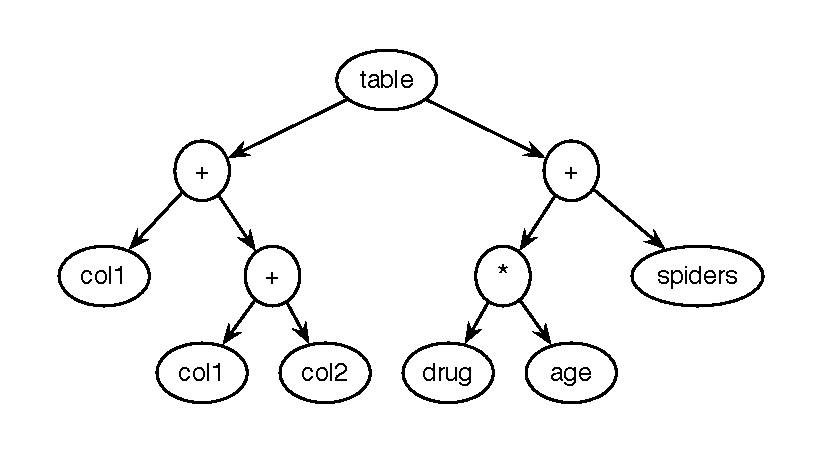
\includegraphics[scale=0.5]{ast1.eps}
    \end{figure}
  \end{frame}      

  \begin{frame}
    \frametitle{Compiling}
    The AST is combined with the data to compile to an S3 object representing a table.
    \begin{figure}
      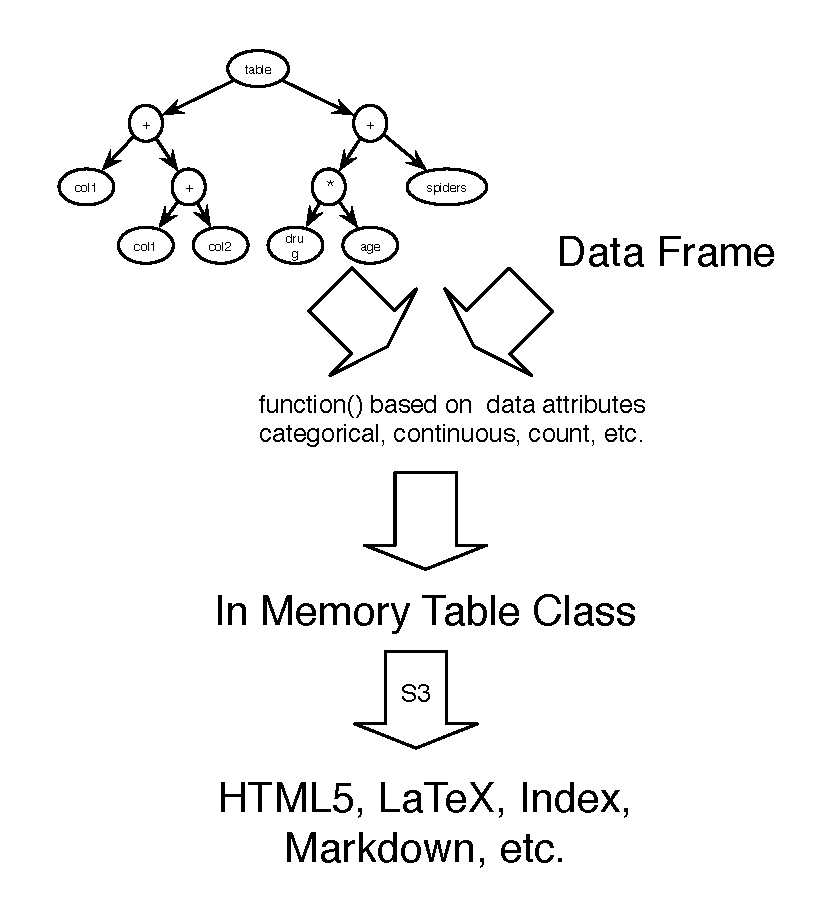
\includegraphics[scale=0.33]{compiler.eps}
    \end{figure}
  \end{frame}      

  \begin{frame}
    \frametitle{Rendering}
    Final rendering is accomplished based on the the S3 call. Any of the intermediate objects in a rendering stack could be overridden by an end user.
  \end{frame}      

  \begin{frame}
    \frametitle{Extensibility}
    Each step of the process to final render can be overridden by the end user, and in a higher surgical manner.
  \end{frame}

  \begin{frame}
    \frametitle{Current Code is on Github}
    See \texttt{spgarbet/reproman} project on \texttt{https://github.com}.


    Feedback?
  \end{frame}
\end{document}
